\section{Language Server}\label{section:prototypische-implementierung:language-server}

\begin{figure}[tbp]
    \centering
    \resizebox{\textwidth}{!}{
        \begin{tikzpicture}
            \begin{class}[text width=7.5cm]{LanguageServerServiceProducer}{0,0}
                \operation{+ sendMessageLSP()}
                \operation{+ onReadFile()}
                \operation{+ onInitialize()}
                \operation{+ onMessageLSP()}
                \operation{+ onFilesystemEvent()}
            \end{class}
            \begin{class}[text width=7.5cm]{LanguageServerServiceConsumer}{8,0}
                \operation{+ initialize()}
                \operation{+ readFile()}
                \operation{+ sendMessageLSP()}
                \operation{+ sendFilesystemEvent()}
                \operation{+ onMessageLSP()}
            \end{class}
        \end{tikzpicture}
    }
    \caption{Klassendiagramm Language Server Service}
    \label{figure:klassendiagramm-language-server-service}
\end{figure}

\begin{figure}[tbp]
    \centering
    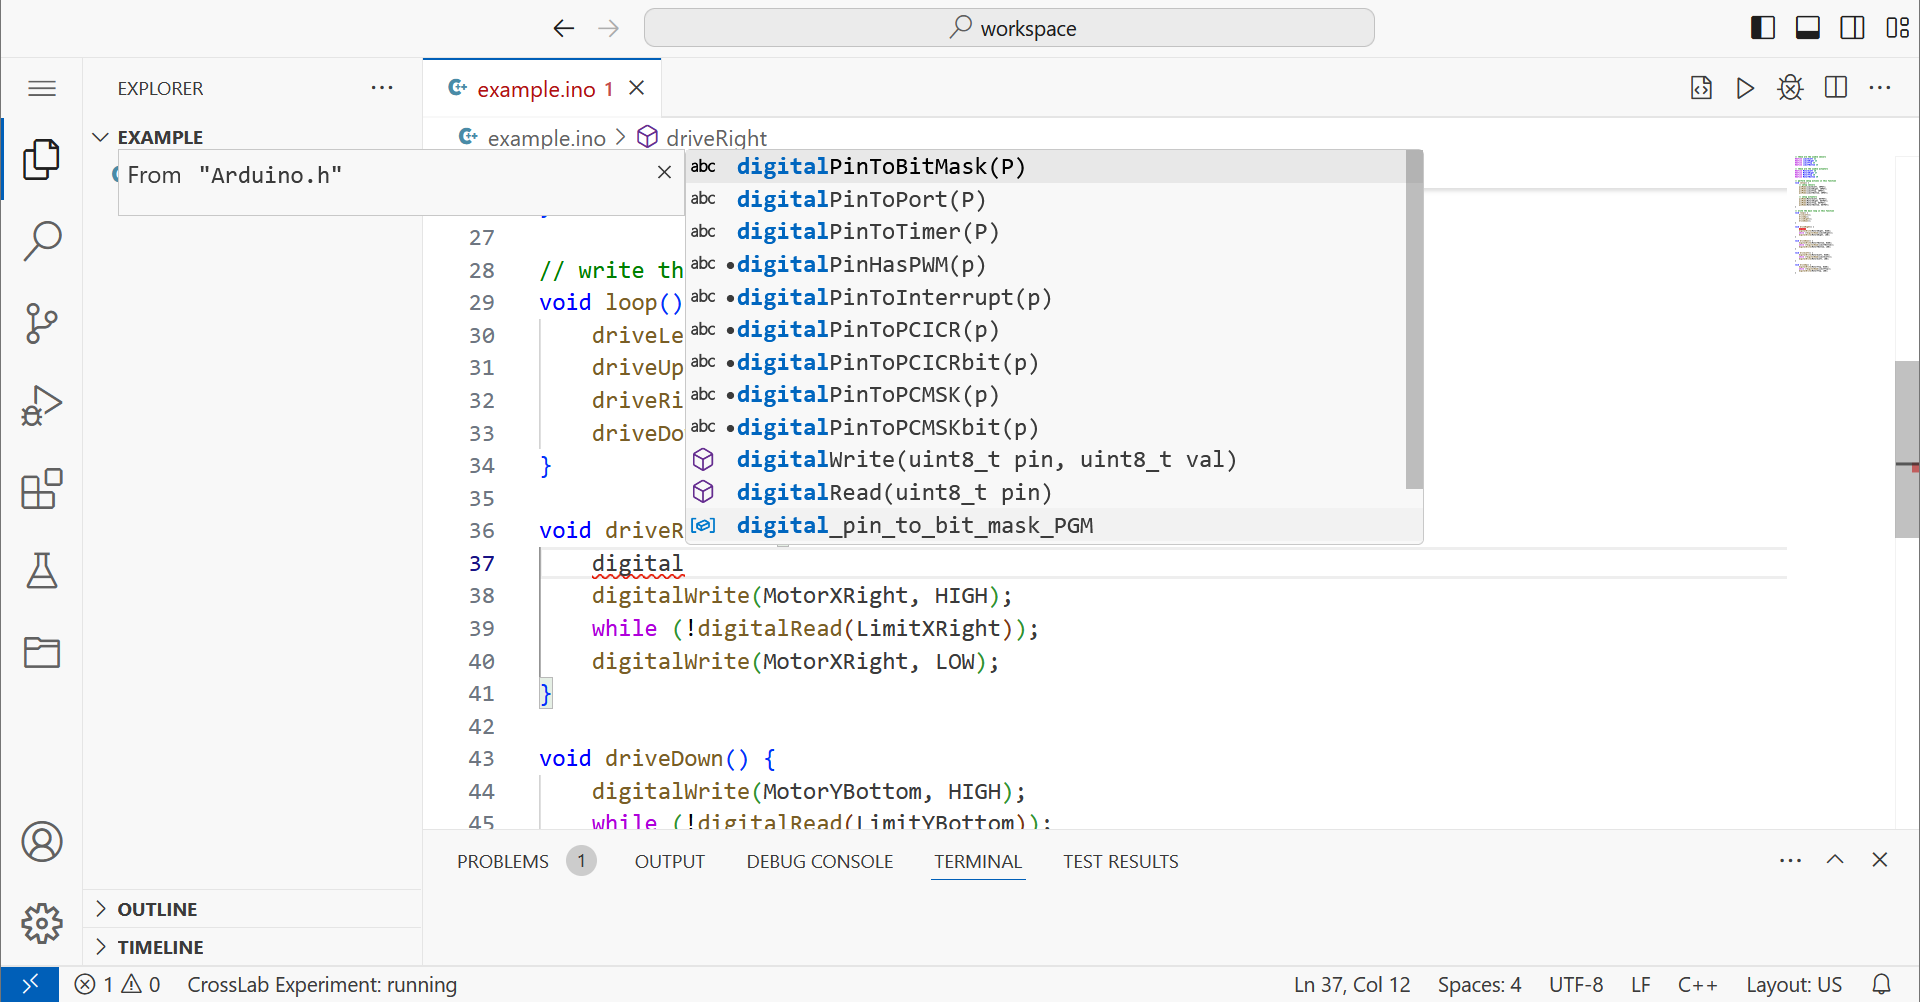
\includegraphics[trim={0 0 0 0},clip,width=\textwidth]{images/language-server.png}
    \caption{Vorschläge des Arduino Language Servers}
    \label{figure:benutzerinterface:language-server}
\end{figure}

Für die prototypische Implementierung wurde ein cloud-instanziierbares Laborgerät für die Bereitstellung des \textit{Arduino Language Servers} \cite{noauthor_arduino-language-server_2025} implementiert. In \autoref{figure:klassendiagramm-language-server-service} ist ein Klassendiagramm für den Language Server Service dargestellt. Wenn die IDE den Language Server startet, schickt sie zunächst mithilfe von \texttt{initialize()} eine entsprechende Initialisierungsnachricht an den Language Server mit dem aktuellen Projekt des Nutzers. Dieses wird auf der Seite des Language Server gespeichert. Danach wird der Language Server gestartet und eine Antwort an die IDE gesendet. Diese kann daraufhin mit der Ausführung des \ac{LSP} beginnen. Dabei muss auf der Seite des Language Servers eine Anpassung der URIs für eingehende und ausgehende \ac{LSP} Nachrichten erfolgen. Dies kann auf eine ähnliche Weise erfolgen, wie es bereits in \autoref{section:prototypische-implementierung:debugging} für das \ac{DAP} beschrieben wurde. Sowohl der Language Server Service Consumer als auch der Language Server Service Producer besitzen Funktionen zum Austausch von LSP Nachrichten. Weiterhin kann der Language Server Service Consumer Dateien mit \texttt{readFile()} anfragen und mit \texttt{sendFilesystemEvent()} Dateisystem-Events an den Language Server Service Producer weiterleiten. Dieser löst entsprechende Events aus, die über Event-Handler behandelt werden können.

Für die IDE wurde eine entsprechende Erweiterung entwickelt. Diese wird im Folgenden als \textit{Language Server Erweiterung} bezeichnet und stellt einen Language Server Service Consumer bereit. Wenn eine Verbindung für diesen besteht, wird der entsprechende Language Server gestartet und über den VSCode Language Client angebunden. Weiterhin wurde ein \texttt{TextDocumentContentProvider} implementiert, der in Verbindung mit dem Language Server Service Consumer den Lesezugriff auf die lokalen Dateien des Language Servers ermöglicht. In \autoref{figure:benutzerinterface:language-server} ist die vom Arduino Language Server angebotene Code-Vervollständigung beispielhaft dargestellt.

Die betrachtete Experimentkonfiguration wird um das neue Laborgerät für die Bereitstellung des Arduino Language Servers erweitert. Dieses wird über den Language Server Service mit den IDEs verbunden (siehe \autoref{figure:experimentkonfiguration:language-server}).